%%%%%%%%%%%%%%%%%%%%%%%%%%%%%%%%%%%%%%%%%%%%%%%%%%%%%%%%%%%%%%%%
% %
% Seth Cram %
% ECE351 Section 53 %
% Prelab 6 %
% Due 02/22/2022 %
% Any other necessary information needed to navigate the file %
%
%
% %
%%%%%%%%%%%%%%%%%%%%%%%%%%%%%%%%%%%%%%%%%%%%%%%%%%%%%%%%%%%%%%%%
%%%%%%%%%%%%%%%%%%%%%%%%%%%%%%%%%%%%%%%%%%%
%%% DOCUMENT PREAMBLE %%%
\documentclass[12pt]{report}
\usepackage[english]{babel}
%\usepackage{natbib}
\usepackage{url}
\usepackage[utf8x]{inputenc}
\usepackage{amsmath}
\usepackage{graphicx}
\graphicspath{{images/}}
\usepackage{parskip}
\usepackage{fancyhdr}
\usepackage{vmargin}
\usepackage{listings}
\usepackage{hyperref}
\usepackage{xcolor}
\usepackage{verbatim}
\usepackage{attachfile}

\definecolor{codegreen}{rgb}{0,0.6,0}
\definecolor{codegray}{rgb}{0.5,0.5,0.5}
\definecolor{codeblue}{rgb}{0,0,0.95}
\definecolor{backcolour}{rgb}{0.95,0.95,0.92}

\begin{comment} %have to use verbatim package for this

\section{Personal Notes}
            


\end{comment}

\lstdefinestyle{mystyle}{
    backgroundcolor=\color{backcolour},   
    commentstyle=\color{codegreen},
    keywordstyle=\color{codeblue},
    numberstyle=\tiny\color{codegray},
    stringstyle=\color{codegreen},
    basicstyle=\ttfamily\footnotesize,
    breakatwhitespace=false,         
    breaklines=true,                 
    captionpos=b,                    
    keepspaces=true,                 
    numbers=left,                    
    numbersep=5pt,                  
    showspaces=false,                
    showstringspaces=false,
    showtabs=false,                  
    tabsize=2
}
 
\lstset{style=mystyle}

\setmarginsrb{3 cm}{2.5 cm}{3 cm}{2.5 cm}{1 cm}{1.5 cm}{1 cm}{1.5 cm}

\title{Lab 5}		%TITLE						
% Title
\author{ Seth Cram}						
% Author
\date{02/15/2022}
% Date

\makeatletter
\let\thetitle\@title
\let\theauthor\@author
\let\thedate\@date
\makeatother

\pagestyle{fancy}
\fancyhf{}
\rhead{\theauthor}
\lhead{\thetitle}
\cfoot{\thepage}
%%%%%%%%%%%%%%%%%%%%%%%%%%%%%%%%%%%%%%%%%%%%
\begin{document}

%%%%%%%%%%%%%%%%%%%%%%%%%%%%%%%%%%%%%%%%%%%%%%%%%%%%%%%%%%%%%%%%%%%%%%%%%%%%%%%%%%%%%%%%%



%%%%%%%%%%%%%%%%%%%%%%%%%%%%%%%%%%%%%%%%%%%%%%%%%%%%%%%%%%%%%%%%%%%%%%%%%%%%%%%%%%%%%%%%%

%%%%%%%%%%%%%%%%%%%%%%%%%%%%%%%%%%%%%%%%%%%%%%%%%%%%%%%%%%%%%%%%%%%%%%%%%%%%%%%%%%%%%%%%%
\renewcommand{\thesection}{\arabic{section}}

Seth Cram \\
ECE351 \\
Prelab 6\\ 
due: 2/22/2022
 
 1. By hand, find the transfer function. Assume all initial conditions are zero. \\
    \begin{equation*}
        H(s) = Y(s)/X(s) = (s^2+6s+12)/((s+4)(s+6))
    \end{equation*}

2. For the system H(s), find y(t) for a step input using partial fraction expansion and inverse
Laplace transforms.
    \begin{equation*}
        y(t) = (0.5 - 0.5 \cdot e^{-4t} + e^{-6t}) \cdot u(t)
    \end{equation*}

    The work gone through to find these two equations is detailed on the following pages.

\newpage


    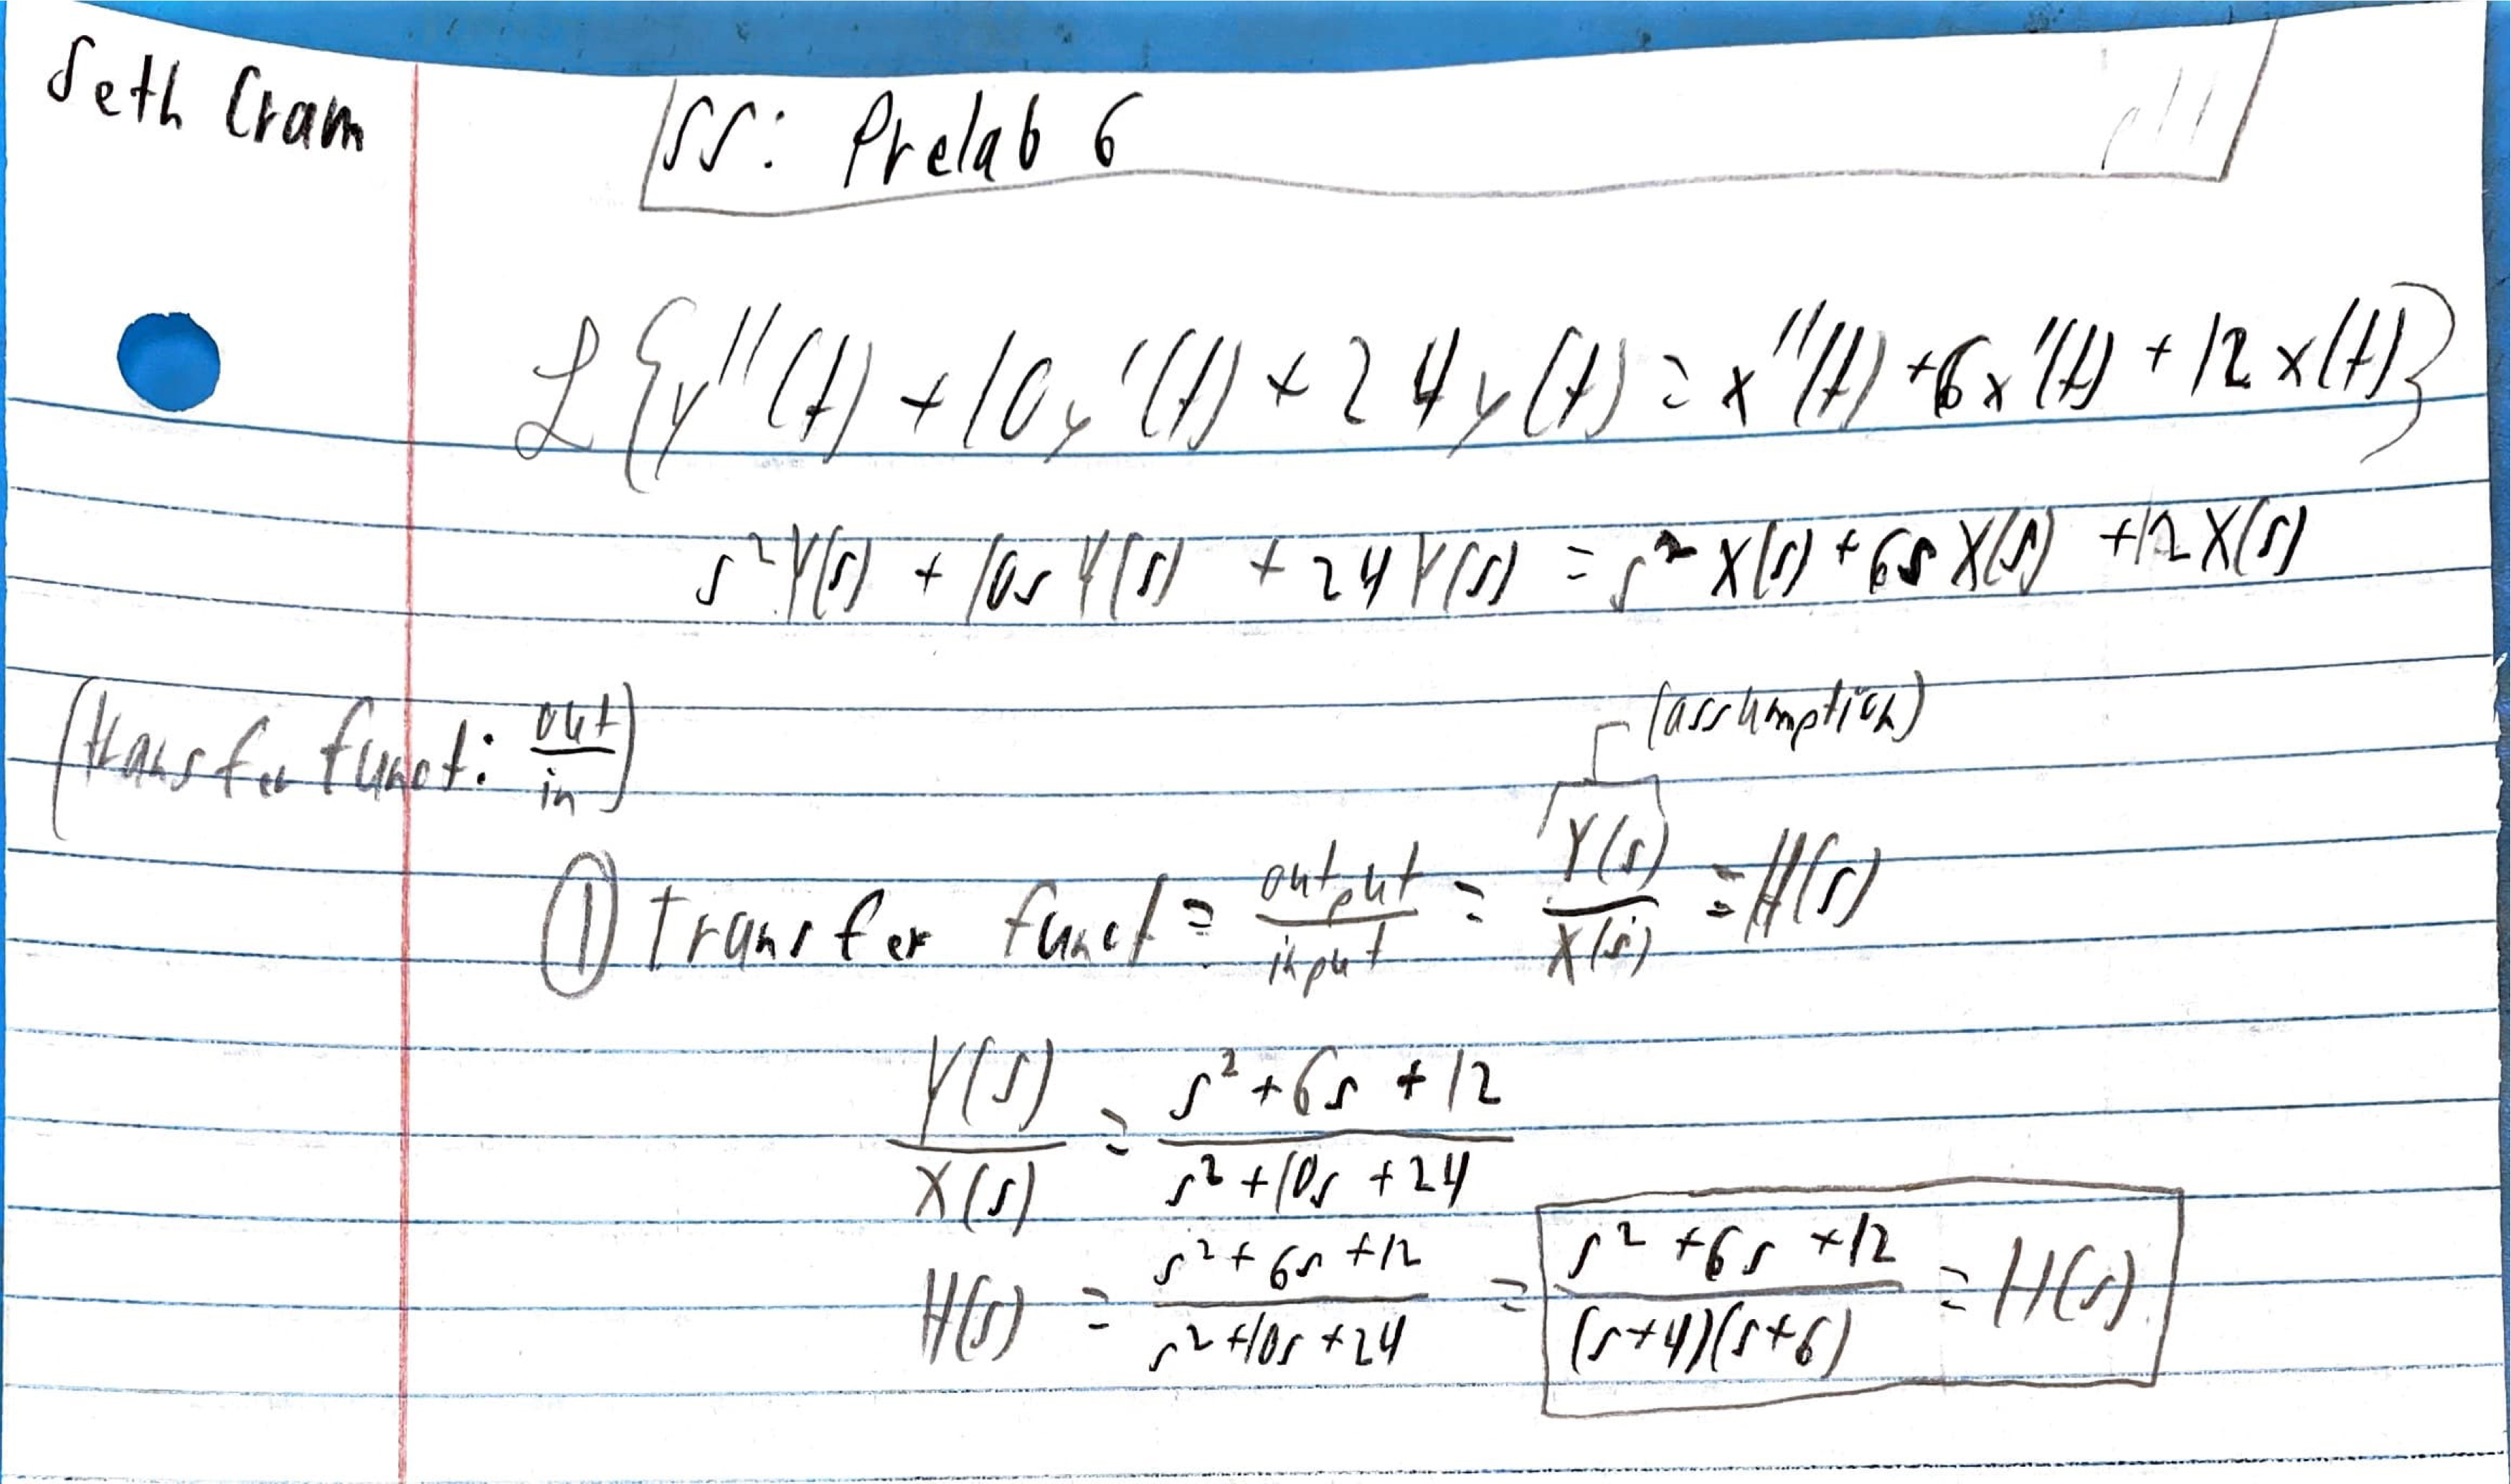
\includegraphics[scale = 0.1]{8283DE04-59E7-407A-96C0-75A20A362B8B.jpeg}

    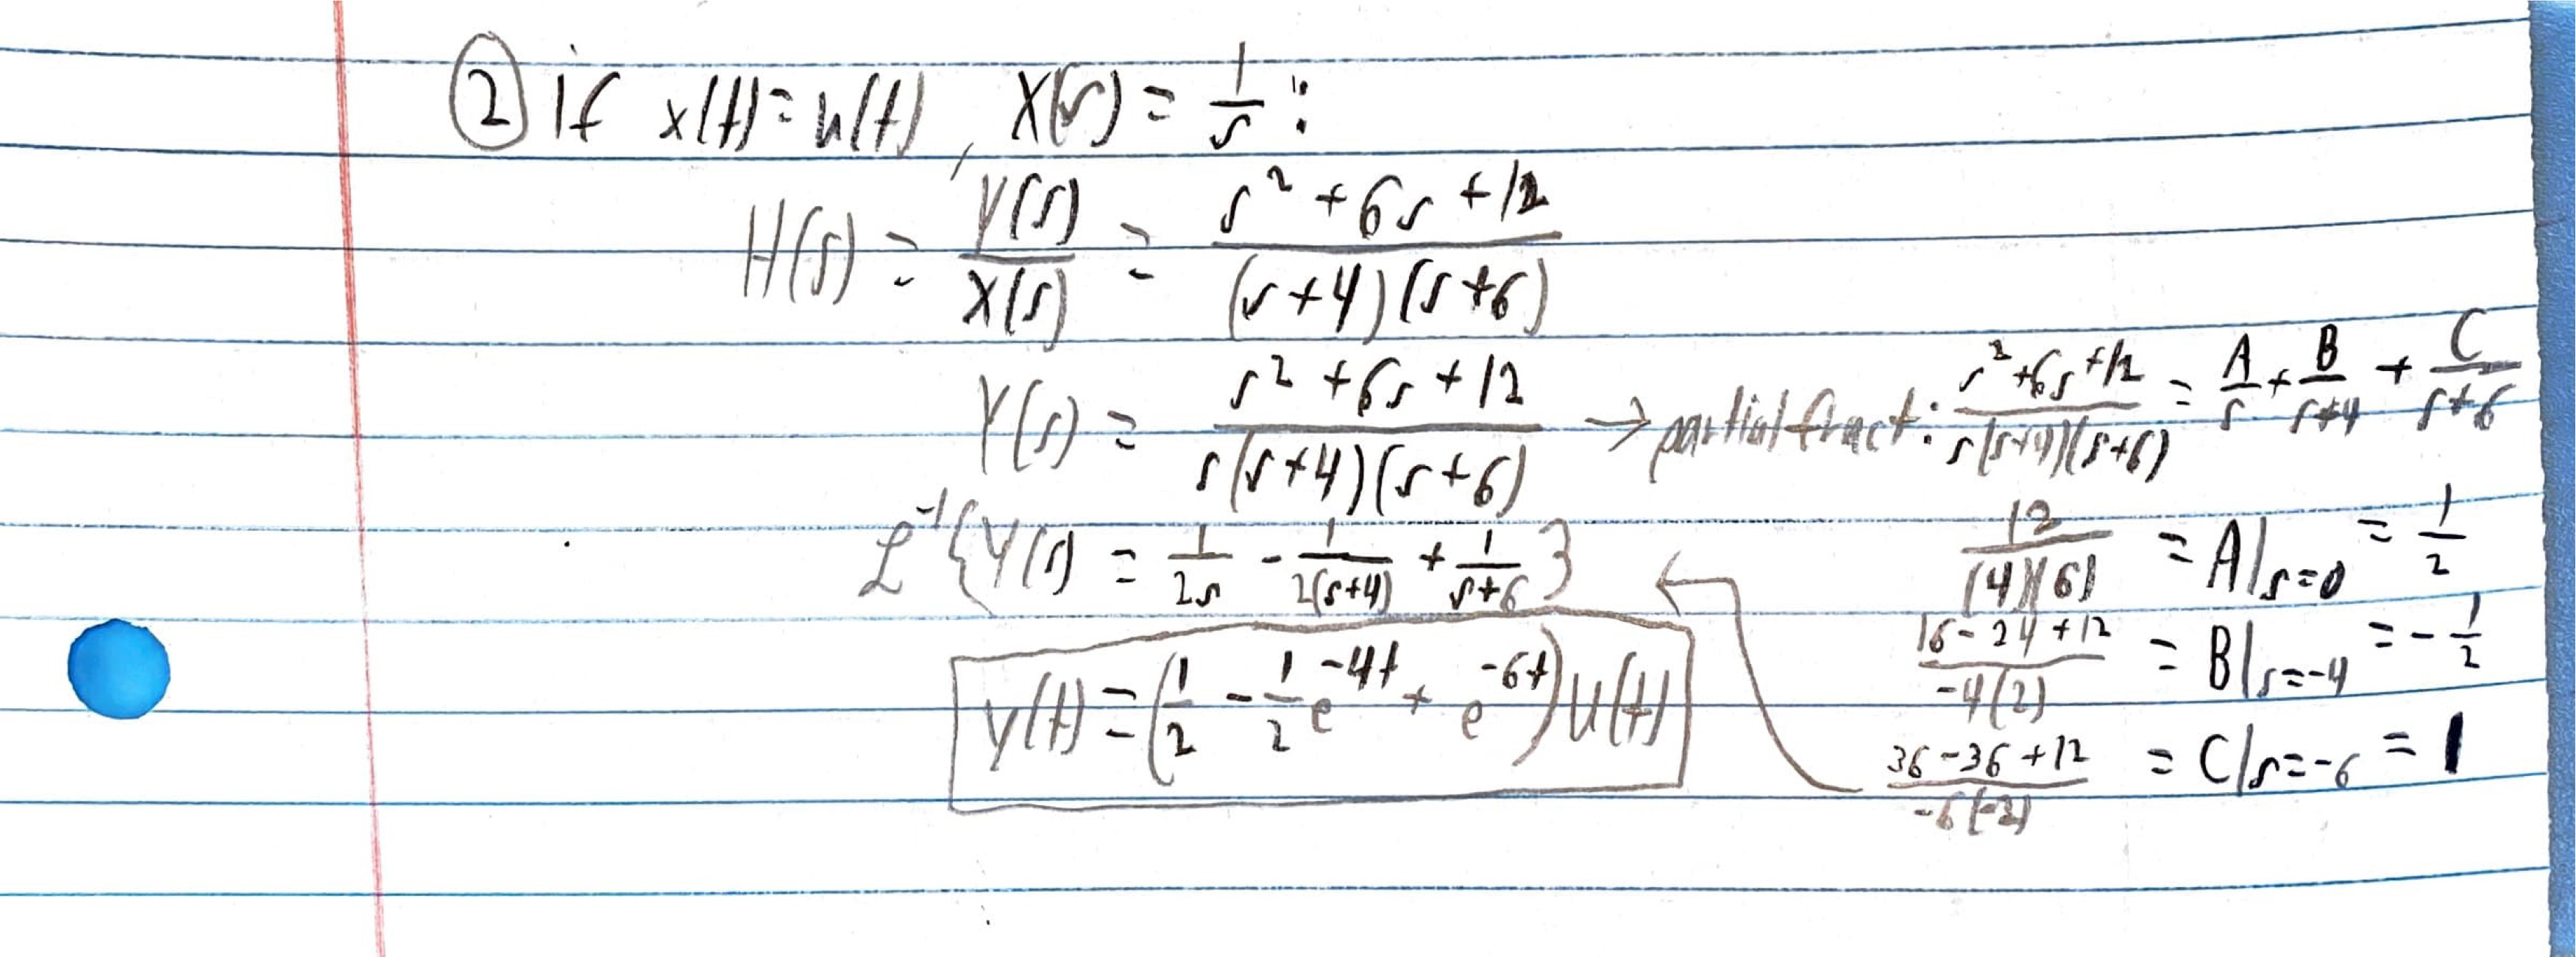
\includegraphics[scale = 0.1]{E6102702-450E-4D2E-81AD-9F1A6F712BC5.jpeg}


    \paragraph{} We can see above how I derived the equations shown on page 1.  

\end{document}